\subsection{Sequence Diagram}
\vspace{2cm}
\begin{figure}[H]
\centering
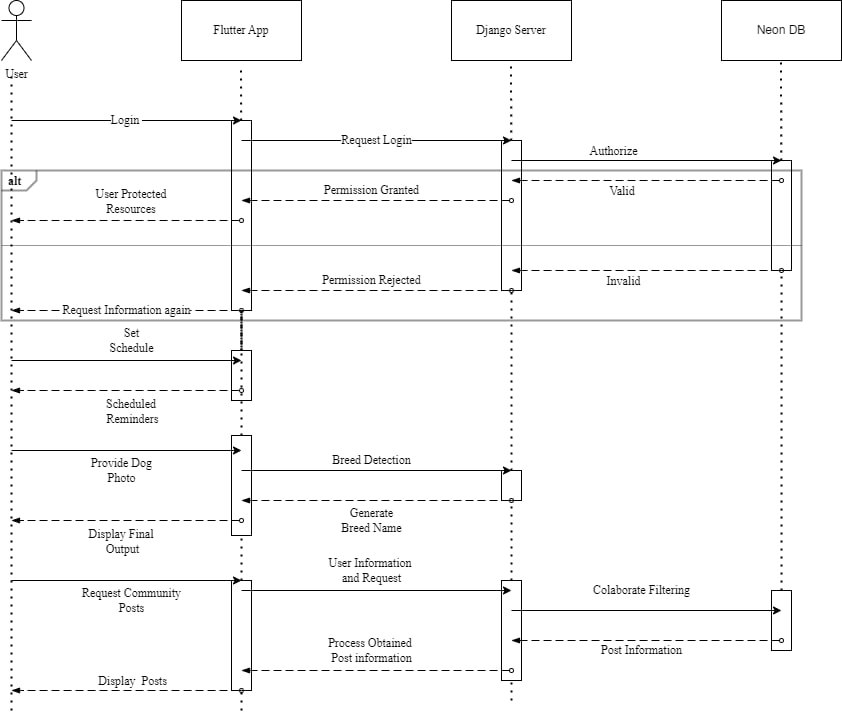
\includegraphics[width=1.01\linewidth]{img/sequencial_diagram.jpg}
\caption{Sequence diagram}
\label{fig:activity-user}
\end{figure}
    \noindent\textbf{User Interaction}\\
        The process begins with a User who initiates interaction by logging in to the HelloPet app.

    \noindent\textbf{Authentication and Authorization}\\
        The Flutter App communicates with the Django Server to send a login request.
        The Django Server authorizes the request, granting or rejecting permission to access protected resources.
        If permission is granted, the user proceeds to the next steps; otherwise, access is denied.

    \noindent\textbf{User Actions}\\
        The user can perform various actions:
            Request Information: The user can request information related to pets or other features.
            Set Schedule: The app allows users to set schedules for pet-related tasks.
            Scheduled Reminders: The app sends scheduled reminders,  care instructions.

    \noindent\textbf{Breed Detection}\\
        When the user provides dog photos, the app processes them for breed detection.
        The Django Server collaborates with the Neon DB to identify the breed of the dog.

    \noindent\textbf{Final Output}\\
        The detected breed name is generated and displayed to the user.
        Additionally, the app may show community posts related to pet care or other relevant topics.